\documentclass{article}

\usepackage[utf8]{inputenc}
\usepackage{graphicx}
\usepackage{fancyhdr}
\usepackage{lastpage}
\usepackage{booktabs}
\usepackage{multirow}
\usepackage{array}
\usepackage[table]{xcolor}
\usepackage{scrextend}
\usepackage{enumitem}
\usepackage{hyperref}
\usepackage{float}


\renewcommand*\rmdefault{iwona}
\renewcommand{\contentsname}{Indice}
\newcommand\tab[1][1cm]{\hspace*{#1}}\newcommand{\parnosep}[1]{\vspace*{-\baselineskip}\paragraph{#1}}
\newcommand{\subparnosep}[1]{\vspace*{-\baselineskip}\subparagraph{#1}}
\renewcommand{\labelenumii}{\theenumi\theenumii.}
\renewcommand{\theenumii}{.\arabic{enumii}}
\renewcommand{\labelenumiii}{\theenumi\theenumii\theenumiii.}
\renewcommand{\theenumiii}{.\arabic{enumiii}}
\newcommand{\nomeprogetto}[0]{B-Party}

\pagestyle{fancy}
\fancyhf{}
\rfoot{Pagina \thepage \hspace{1pt} di \pageref{LastPage}}

%Copertina e Indice
\title{\textbf{Relazione su Frequent Itemsets Mining\\}}
\date{\today}
\author{ \textit{Fontolan Federico} 854230\\\textit{Rosada Fabio} 851772\\}

\begin{document}
\pagenumbering{gobble}
\maketitle
\begin{figure}[t!]
  \begin{center}
  
\includegraphics[width=200px]{logo_ca_foscari.jpg}
  \end{center}
\end{figure}
\vfill
\newpage


\pagenumbering{arabic}

\section{Introduzione}
L'esercitazione che ci è stata assegnata prevedeva di implementare un algoritmo che prendesse in analisi dieci milioni di tweet e ritornasse i frequent itemsets; il nostro gruppo ha deciso di implementare un algoritmo random sampling perché la grande mole dei dati permette di raggiungere risultati soddisfacenti anche solo analizzandone una parte relativamente piccola come il 10\% senza compromettere la validità dei dati essendo lo stesso campione estremamente grande.\\
Il core del nostro codice è stato scritto nella sua interezza in simultanea dai membri del gruppo, alternandosi nella scrittura come previsto nella tecnica del "pair programming". La revisione finale del codice con la riscrittura dei commenti e l'eliminazione delle righe superflue è stata affidata a Fabio Rosada, mentre la scrittura di questa relazione a Federico Fontolan.

\section{Scelte Fatte nella Stesura del Codice}

Il nostro codice all'avvio, dopo avere stampato i dettagli del settaggio corrente (sample, threshold e file di input), genera uno SparkContext e carica in memoria la lista di stopwords che servirà per la rimozione delle stesse: la peculiarità di queste parole è quella di essere estremamente ricorrenti, quindi ogni itemset che le contenga sarà di scarso interesse.\\
Successivamente leggiamo ed estraiamo un sample con la combinazione delle funzioni textFile() e sample() e generiamo una lista rappresentante il contenuto dei bucket: questa scelta permette di limitare il numero di letture del file che è la parte tempisticamente più onerosa permettendoci di eseguire l'intero programma in meno di dieci minuti. Nel file è comunque presente sotto forma di commento una versione funzionante del software che legge i file ogni volta questo sia necessario per eliminare lo spazio occupato da questa lista che però causa un abbattimento generale delle prestazioni.\\
La lettura dei tweet viene effettuata considerando i tweet come testo e non come json: questo scelta è dovuta alla lentezza nell'elaborazione del file con il secondo metodo riscontratasi nella fase di test.
Finita questa fase viene eseguito un algoritmo apriori che continua a ricercare itemsets finché esiste almeno un itemset di rango inferiore: questo è dovuto al principio di monotonicità.
\newpage
\section{Risultati}
NOTA: le funzioni per sinteticità mostrano i primi 20 risultati ordinati per frequenza, ma è possibile visualizzarli cambiando i valori di input nel codice.

\begin{figure}[h]
  \begin{center}
  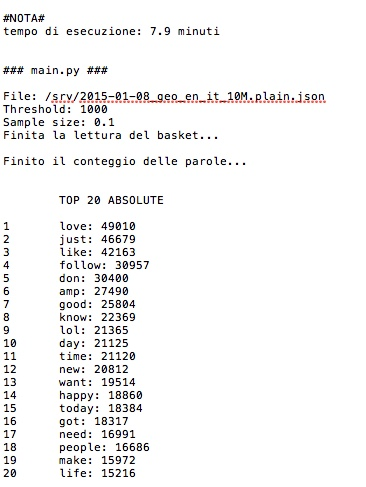
\includegraphics[width=300px]{1code.jpeg}
  \end{center}
\end{figure}


\newpage
\begin{figure}[h]
  \begin{center}
  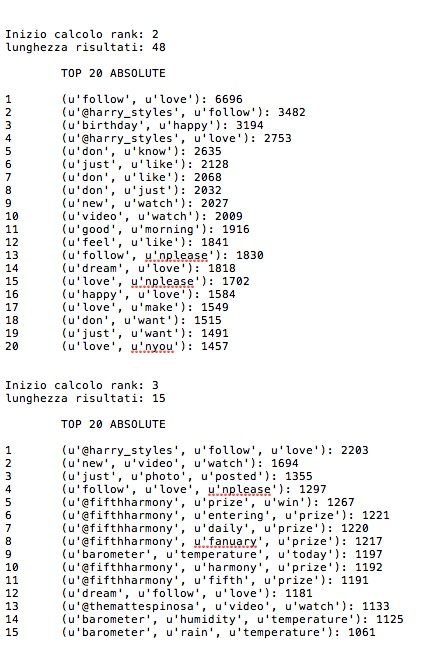
\includegraphics[width=250px]{2code.jpeg}
  \end{center}
\end{figure}

\newpage
\begin{figure}[h]
  \begin{center}
  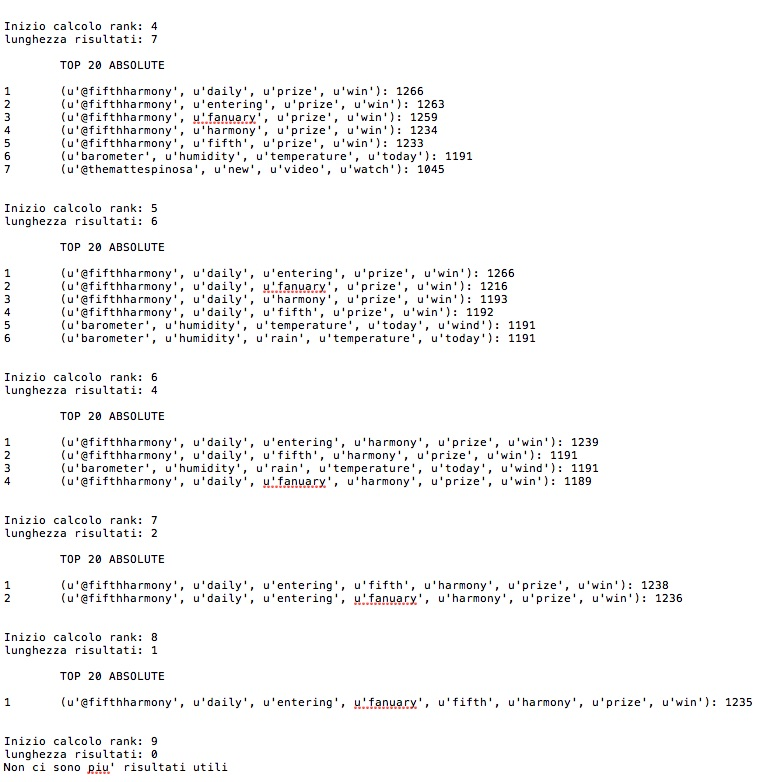
\includegraphics[width=300px]{3code.jpg}
  \end{center}
\end{figure}



\paragraph{Commenti}
Per questo esperimento è stato scelto un threshold molto basso(lo 0.001) per permettere di ottenere anche un buon numero di tuple di rango superiore al 2.\\
Nel corso di vari testi sia con il file maggiore sia con quello minore abbiamo notato che alcune particolari tuple molto lunghe compaiono un numero molto elevato di volte: questo fenomeno succede se un tweet viene retwettato un numero di volte superiore al threshold.
\newpage
\section{Confronto}
\begin{figure}[h]
  \begin{center}
  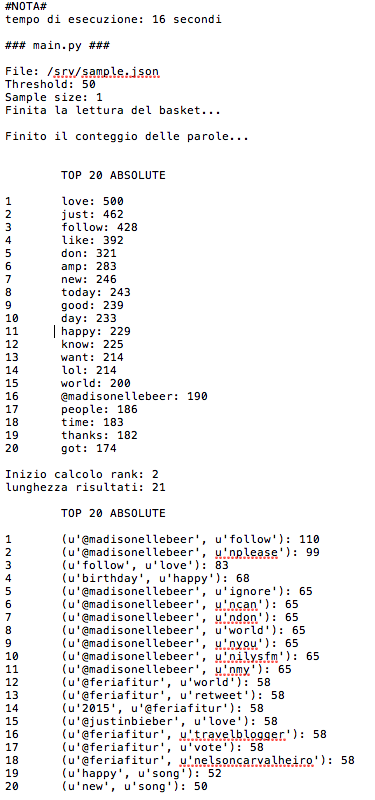
\includegraphics[width=190px]{sample1.jpg}
  \end{center}
\end{figure}


\begin{figure}[h]
  \begin{center}
  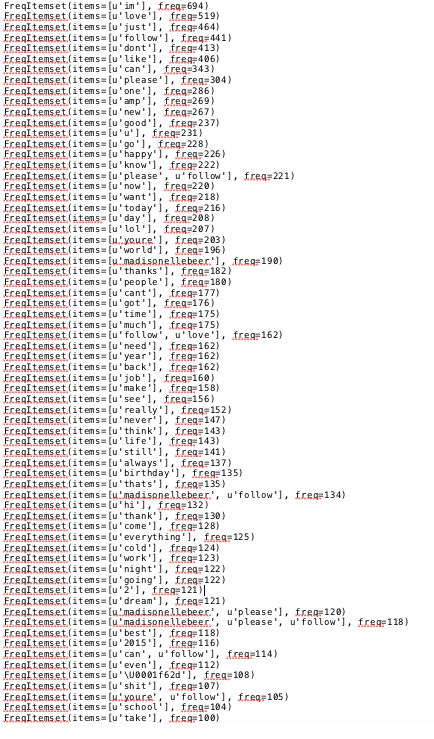
\includegraphics[width=190px]{samplefp}
  \end{center}
\end{figure}



\paragraph{Risultati} La fase di confronto è stata eseguita con sul file da diecimila tweet e concentriamo la nostra attenzione fino al rango due dei risultati trovati dal nostro software.
Si può notare che le parole frequenti individuate (escluse stopwords) sono le stesse, anche sono un valore leggermente inferiore dovuto al sistema di pulizia eseguito sulla stringa. 
Il nostro software è leggermente più veloce (circa 2-3 secondi) rispetto a fpgrowth con il file piccolo.




\end{document}
